\documentclass[12pt]{article}

\usepackage[utf8x]{inputenc}
\usepackage{ucs}
\usepackage{color}
\usepackage{indentfirst}
\usepackage{mathtools}
\usepackage{amsmath}
\usepackage{amsfonts}
\usepackage{amsthm}
\usepackage{amssymb}
\usepackage{enumerate}
\usepackage{listings}
\usepackage{hyperref}
\usepackage{float}
\usepackage{url}
\usepackage{enumitem}
\usepackage[margin=1in]{geometry}
\usepackage[nottoc,numbib]{tocbibind}
\usepackage{combelow}
\usepackage{amsfonts}
\usepackage{multicol}
\usepackage{graphicx}
\usepackage{subcaption}

\setlength{\parskip}{2ex plus 0.5ex minus 0.2ex}
\setcounter{secnumdepth}{2}
\setcounter{section}{-1}
\setlist{nolistsep}

\newcommand{\ddaca}{\Leftrightarrow}
\newcommand{\then}{\Rightarrow}

\newcommand\blfootnote[1]{%
  \begingroup
  \renewcommand\thefootnote{}\footnote{#1}%
  \addtocounter{footnote}{-1}%
  \endgroup
}

\newtheorem{thr}{\bf Teorem\u{a}}[section]
\newtheorem{cor}[thr]{\bf Corolar}
\newtheorem{lema}[thr]{\bf Lem\u{a}}
\newtheorem{prob}[thr]{\bf Problem\u{a}}
\newtheorem{obs}[thr]{\bf Observa\c{t}ie}
\newtheorem{ex}[thr]{\bf Exemplu}
\newtheorem{exs}[thr]{\bf Exemple}
\theoremstyle{definition}
\newtheorem{defi}[thr]{\bf Defini\c{t}ie}
\newtheorem{thr-defi}[thr]{\bf Teorem\u{a}-Defini\c{t}ie}
\newtheorem{nota}[thr]{\bf Nota\cb{t}ie}
\thispagestyle{empty}

\title{Colorizarea pozelor alb-negru}
\date{}
\author{Eric Petru Stavarache, Lucian Bicsi}

\begin{document}

\maketitle

\tableofcontents


\begin{abstract}
    Aceasta lucrare trateaza colorizarea pozelor folosind retele adversariale generative, in particular arhitecturile CycleGAN si StarGAN.

    Scopul lucrarii este de a testa capacitatea de invatare a retelelor pe problema colorizarii in particular si de a o compara cu abordarile traditionale.
\end{abstract}

\section{Introducere}

Colorizarea pozelor alb-negru este o sarcina dificila pentru metodele traditionale de invatare.

Una dintre cele mai mari contributii la aceasta dificultate o aduce faptul ca retele traditionale sunt specializate pe minimizarea unei pierderi de tipul $log-loss$ sau $L2$.
Consideram spatiul 3-dimensional al culorilor pixelilor RGB: $\{0, 1, ..., 255 \}^{3}$. Punctele care minimizeaza suma distantelor $L2$ tind sa fie distribuite in jurul mediei distributiei intensitatii, astfel rezultand poze preponderent in tonuri de gri, lipsite de culori.

\section{Munca Anterioara}

Abordarea clasica de colorizare a pozelor este bazata pe retele convolutionale, iar rezultatele din 2016 ale lui Richard Zhang et al sunt impresionante [1][2].
Pentru a rezolva problema distributiei culorilor, autorii propun modificarea functiei de pierdere pentru a penaliza culorile care nu apar frecvent in poze.
i.e., desi culoarea gri minimizeaza $L2-loss$, nu este intalnita foarte des in pozele adevarate, deci nu va mai fi culoare dominanta in pozele colorizate.


\section{Preliminarii}

\subsection{Notiuni generale}

\begin{subsubsection}{Retele generative adversariale}
\begin{defi}
Retelele generative adversariale (eng. Generative Adversarial Network) au fost inventate de catre Ian Goodfellow in 2014.
Acestea sunt cea mai noua metoda de a rezolva problema esantionarii dintr-un spatiu al datelor unde abordarile traditionale au un bias catre medie. [5].

Aceste retele sunt compuse din doua parti: reteaua generatoare si reteaua discriminatoare.
Reteaua generatoare $G$ incearca sa genereze output din distrubtia $\mathcal{O}$, bazandu-se fie pe input din distributia $\mathcal{I}$. Vom nota distributia lui $G$ cu $\mathcal{G}$.
Reteaua discriminatoare $D$ consta intr-un \textbf{clasificator (binar)} care primeste ca input o poza $i \in \mathcal{I}$ si incearca sa distinga daca $i$ a provenit din $\mathcal{O}$, distributia adevarata a datelor, sau din $\mathcal{G}$, distributia pe care o genereaza $G$.

Indicele de performanta al retelei $G$ este data de cat de bine reuseasca sa "pacaleasca" reteaua $D$, in timp ce performanta retelei $D$ este cat de bine reuseste sa distinga intre datele adevarate si cele artificiale. Retelele vor fi antrenate in paralel, in decursul a mai multor epoci.

\end{defi}
Motivatia centrala din spatele acestui tip de model isi are originile in \textbf{teoria jocurilor}. Retelele $G$ si $D$ pot fi vazuti ca doi adversari intr-un joc de tip min-max: $G$ incearca sa maximizeze scorul, in timp ce $D$ incearca sa minimizeze scorul. Aici scorul este definit ca fiind, spre exemplu, numarul de poze clasificate gresit de catre $D$. De aici provine numele de \textsc{retele adversariale}.

\begin{figure}
  \centering
  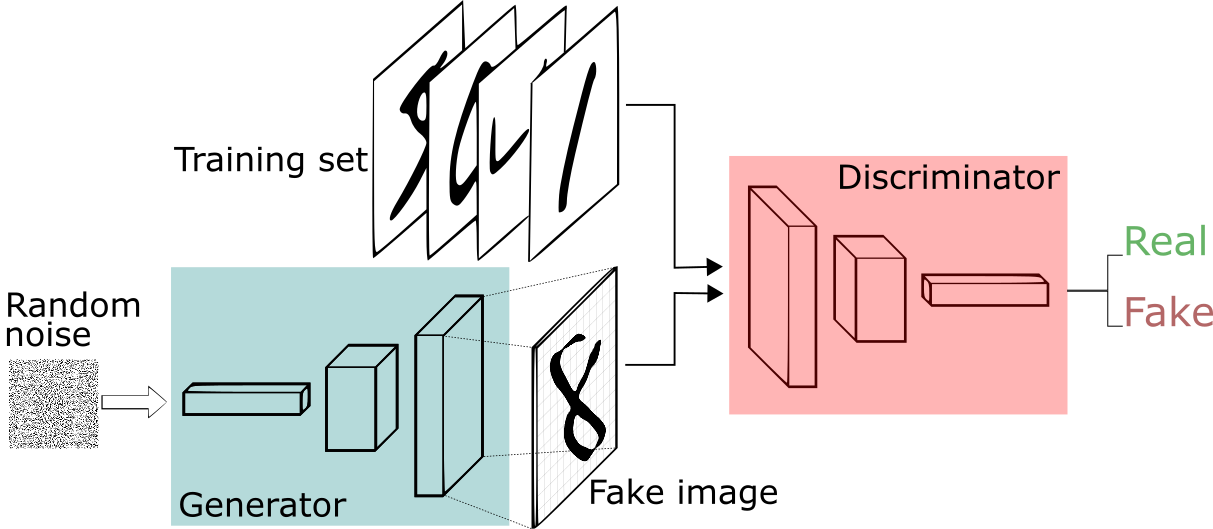
\includegraphics[width=0.7\linewidth]{GAN.png}
  \caption{Retele Adversariale Generative}
  \label{fig:GAN}
\end{figure}

\end{subsubsection}

\subsection{Date de antrenare}

Pentru antrenarea retelei am combinat dataset-urile puse la dispozitie de autorii CycleGAN [6].
Aceste dataset-uri au fost menite pentru a transforma dintr-un domeniu specific in altul (de exemplu de a converti din cai in zebre).
Pentru a spori diversitatea, am creat datasetul prin reuniunea tuturor pozelor puse la dispozitie, deoarece domeniul de poze color include toate celelate poze.
Pentru fiecare poza din reuniune, am generat varianta alb-negru.

\section{Colorizare folosind GAN-uri}

Aceasta lucrare incearca sa trateze problema colorizarii folosind Retele Adversariale Generative - GAN.
Abordarea naiva ar fi formata din cele doua componente clasice: reteaua generatoare si cea discriminatoare.
Reteaua generatoare $G$ primeste o imagine alb-negru si generaza una color.
Reteaua discriminatoare $D$ primeste o imagine color, si incearca sa distinga daca este o imagine naturala, sau daca a fost generata de catre $D$.

Principala problema cu aceasta abordare este ca reteaua generatoare descopera ca optim este sa genereze mereu aceeasi poza colorata, fara a tine cont de input. Pentru a rezolva asta, vom utiliza generatori bidirectionali, idee prezentata in cadrul a doua abordari arhitecturale: prima dintre ele se numeste \textit{Unpaired Image-to-Image Translation using Cycle-Consistent Adversarial Networks}, sau CycleGAN [3][4], iar a doua \textit{Unified Generative Adversarial Networks for Multi-Domain Image-to-Image Translation} sau StarGAN [7][8].

\subsection{CycleGAN}

CycleGAN este un model care rezolva problema ca output-ul generatorului nu depinde de input.
Ideea centrala este sa avem un generator $G1$ care ne trece din domeniul $\mathcal{I}$ in domeniul $\mathcal{G}$ si un generator $G2$ care ne trece din $\mathcal{G}$ in $\mathcal{I}$.
Functiile lor de pierdere vor fi corelate de faptul ca vrem ca transformarea inversa sa fie idempotenta.
i.e., daca din alb-negru trecem o poza in color si apoi inapoi in alb-negru, vrem ca cele doua poze alb-negru sa fie cat de similare se poate.

Evaluarea performantei celor doi generatori va fi facuta de catre doi discriminatori specializati $D1$ si $D2$. Astfel, $D1$ va evalua poze color adevarate vs. poze color false generate de catre $G1$, iar $D2$ va evalua poze alb-negru adevarate vs. poze alb-negru false generate de catre $G2$.

CycleGAN a obtinut rezultate remarcabile in cadrul altor task-uri asemanatoare computational cu cel al colorizarii, precum transformarea cailor in zebre, transformarea peisajelor de vara in iarna, zi - noapte, etc.

\begin{figure}[H]
  \centering

	\begin{subfigure}{0.4\textwidth}
	    \centering
		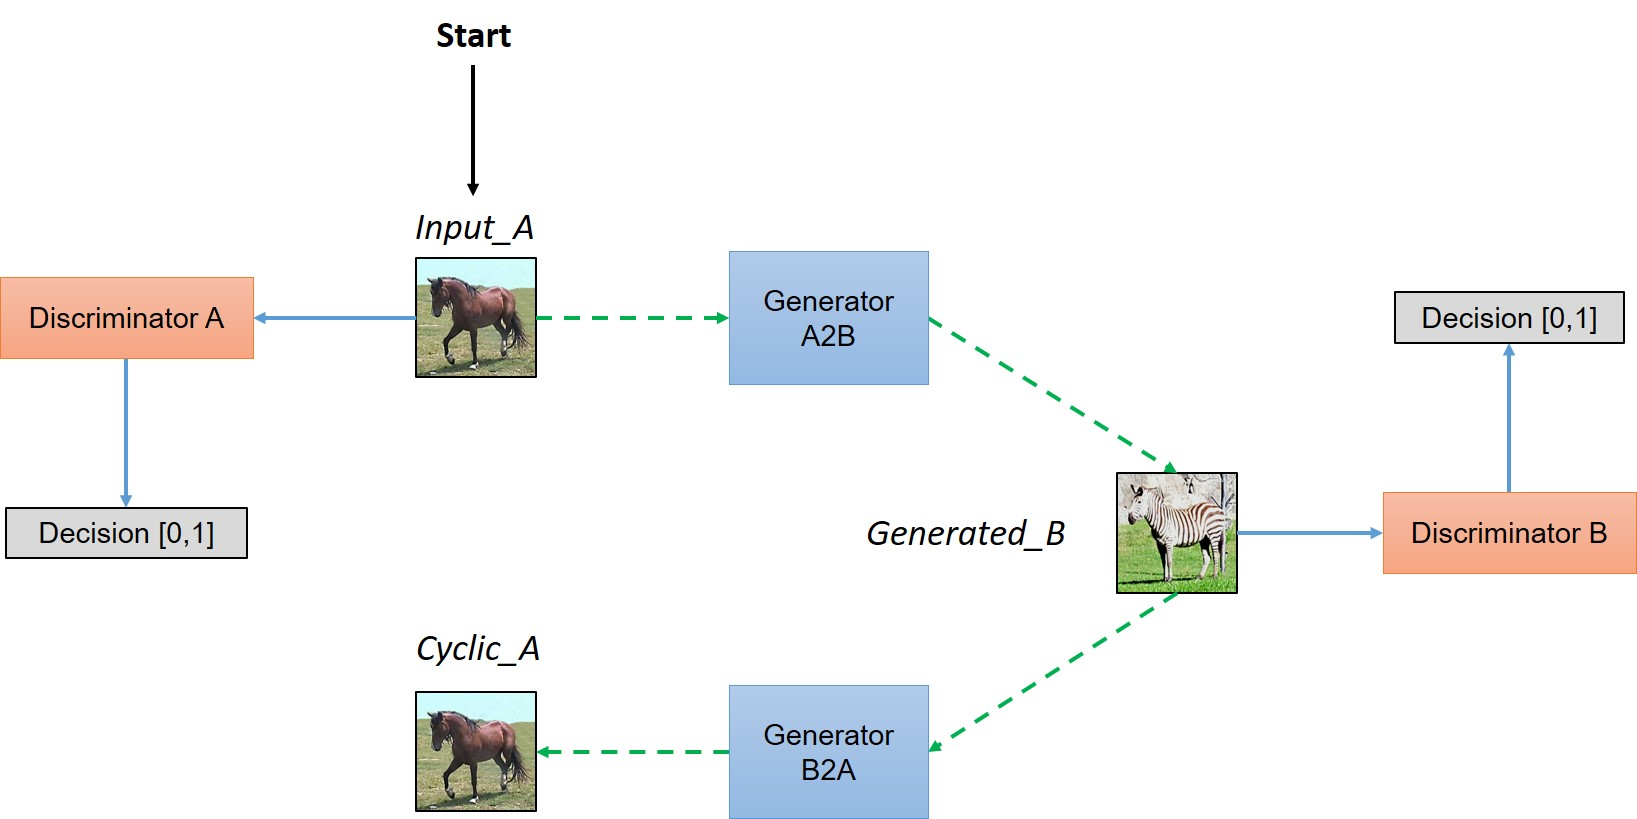
\includegraphics[width=\linewidth]{model.jpg}
		\caption{Ciclul A \Rightarrow B \Rightarrow A}
	\end{subfigure}
	\vspace{1em}
	\begin{subfigure}{0.4\textwidth}
		\centering
		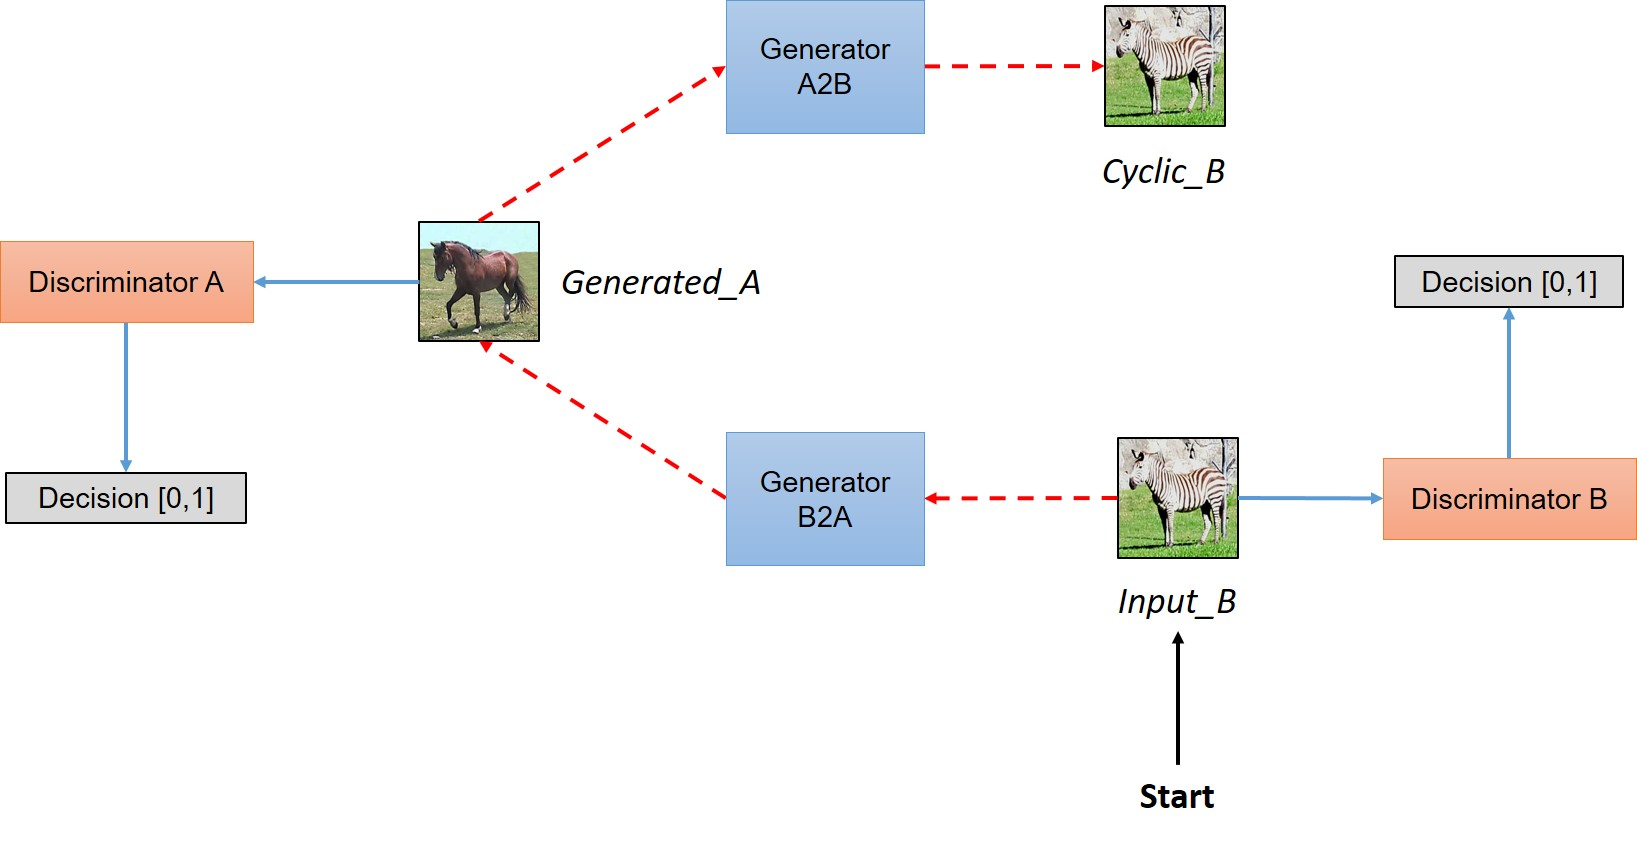
\includegraphics[width=\linewidth]{model1.jpg}
		\caption{Ciclul B \Rightarrow A \Rightarrow B}
	\end{subfigure}

  \caption{Modelul de functionare CycleGAN}
  \label{fig:architecture}
\end{figure}

\subsection{StarGAN}

StarGAN este o retea generativa, construita in original pentru transferul atributelor faciale si pentru a incerca sa reproduca expresii/gesturi faciale corespunzatoare sentimentelor primare (fericire, tristete, dezgust, surprindere, etc.). Strategia este diferita de cea din spatele CycleGAN, in sensul ca prezinta un generator cu functie multipla, in locul celor doi generatori $G1$ si $G2$ mutual inversi ai retelei CycleGAN. Acelasi lucru se intampla si in cadrul disriminatorilor, fiind imbinati intr-unul singur, care nu mai este binar. Arhitectura generatorului este de tip \textbf{encoder-decoder}, in timp ce discriminatorul este un clasificator binar peste o retea convolutionala.

Diferenta principala intre functionalitatile StarGAN comparativ cu CycleGAN este ca StarGAN trateaza problema mai multor clase posibile de domenii, ceea ce nu ne este util in cazul colorizarii propriu-zise, insa se poate folosi daca dorim diverse tipuri de colorizari (sepia, noapte/zi, tonuri calde/reci, etc.). Cu toate acestea, pentru acest lucru este nevoie de un dataset mult mai mare si mai expresiv, de care nu dispunem momentan.

Un mare avantaj in cadrul implementarii pytorch a StarGAN [8] este faptul ca reteaua este puternic customizabila, putand seta hiperparametri precum redimensionarea imaginilor input, setarea numarului de straturi intermediare in cadrul generatorului / discriminatorului, (astfel avand posibilitatea de a testa codul local pe o arhitectura minimala inainte de antrenarea propriu-zisa), setarea intervalului de iteratii la care este salvat modelul, capacitatea de a porni de la un model preantrenat, etc.

\begin{figure}[H]
  \centering

	\begin{subfigure}{0.4\textwidth}
	    \centering
		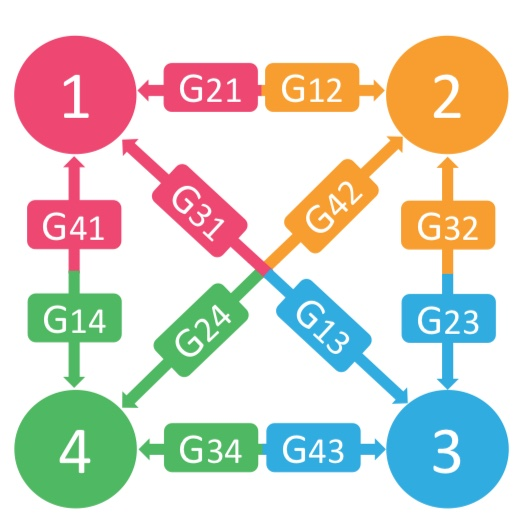
\includegraphics[width=\linewidth]{stargan.jpg}
		\caption{GAN clasic - generator pentru fiecare pereche de clase}
	\end{subfigure}
	\vspace{1em}
	\begin{subfigure}{0.4\textwidth}
		\centering
		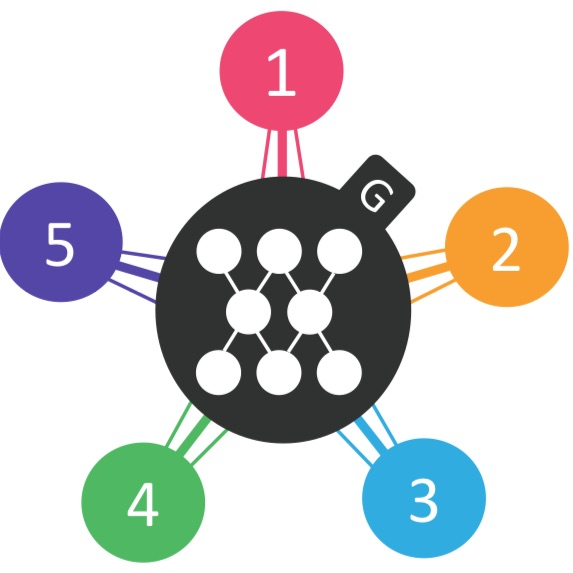
\includegraphics[width=\linewidth]{stargan1.jpg}
		\caption{StarGAN - un singur generator central, conectat in stea}
	\end{subfigure}

  \caption{Modelul de functionare StarGAN}
  \label{fig:architecture}
\end{figure}

\section{Rezultate, concluzii, posibile imbunatatiri}

\subsection{CycleGAN}

Pozele colorizate de catre reteaua CycleGAN sunt satisfacatoare. Comparativ cu metodele de colorizare state-of-the-art, outputul retelei pare incetosat.
Aceste fapt se genereaza cantitatii mici de date de antrenare folosite, iar o posibila imbunatatire ar fi utilizarea setului de antrenare ImageNET.

O alta imbunatatire generala posibila consta, bineinteles, in antrenarea mai multor iteratii si eventual in antrenarea unor retele mai adanci pe o cantitate mai mare de date si cu un numar mai mare de iteratii.

Un alt mod prin care performantele pot fi imbunatatite sunt prin calibrarea mai buna a  hiperparametrilor pe problema specifica a colorizarii.


\begin{figure}[H]
	\centering
	\begin{subfigure}{0.4\textwidth}
		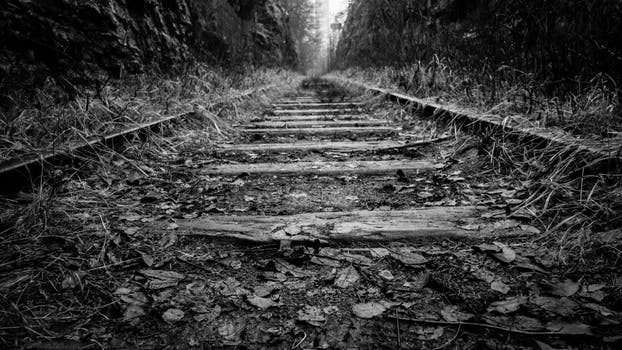
\includegraphics[width=\linewidth]{input_sample.jpg}
		\caption{Poza alb-negru}
	\end{subfigure}
	\vspace{1em}
	\begin{subfigure}{0.4\textwidth}
		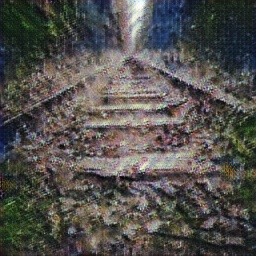
\includegraphics[width=\textwidth]{output_sample.jpg}
		\caption{Poza colorata}
	\end{subfigure}
	\caption{Colorizarea unei poze cu CycleGAN}
\end{figure}

\subsection{StarGAN}

Spre deosebire de rezultatele obtinute de reteaua CycleGAN, reteaua StarGAN, nu a obtinut rezultate la fel de incantatoare. In cadrul procesului de antrenare, calitatea estetica a pozelor generate oscileaza. Reteaua a fost antrenata pe doua dataseturi (apple2orange si summer2winter). Pe pozele din datasetul apple2orange reteaua coloreaza corespunzator doar cateodata, in timp ce pe pozele din datasetul summer2winter, rezultatele sunt mai estetice. Acest lucru se poate datora si faptului ca in cadrul celui de-al doilea dataset exista o gama variata de colorari valide, in timp ce in datasetul apple2orange exista constrangeri mai mari in cadrul colorarii (bineinteles, una dintre acestea fiind paleta limitata de culori - rosu sau portocaliu).

Cu toate acestea, rezultatele obtinute la acest moment nu sunt inca concludente, deoarece reteaua nu a fost antrenata decat pentru o fractiune (~20\%) din iteratiile recomandate de catre autori, iar datasetul nu a fost la fel de expresiv ca in cadrul CycleGAN. Ne asteptam ca, dupa o perioada comparabil de lunga de antrenare, reteaua StarGAN sa obtine rezultate mult mai calitative.

In acelasi timp, o ipoteza de-a noastra este ca problema transferului atributelor faciale, in cadrul careia o transformare [$happy \Rightarrow sad$] si una [$sad \Rightarrow happy$] impart o cantitate foarte mare din informatiile imaginei input (i.e., restul imaginii ramane neschimbat), fapt ce determina ca un generator "shared" sa reuseasca sa codifice informatiile esentiale cu un numar mic de parametri, in timp ce problema colorizarii formalizat in acelasi cadru prezinta diferente uriase la nivel de structura a pozei. In cadrul problemei colorizarii, discriminatorul StarGAN trebuie sa invete dubla functionalitate de colorizare si decolorizare aproximativ independent in cadrul acelorasi parametri. DIn acest motiv, este posibil ca reteaua StarGAN sa fie underfit pentru problema colorizarii.

\section{Bibliografie}

[1] Richard Zang, Phillip Isola, Alexei A. Efros \\ \textit {Colorful Image Colorization}, https://arxiv.org/pdf/1603.08511.pdf, ECCV, 2016. \par
[2] Richard Zang \textit {Colorful Image Colorizaiton}, http://richzhang.github.io/colorization/ \par
[3] Jun-Yan Zhu, Taesung Park, Phillip Isola, Alexei A. Efros, \textit {Unpaired Image-to-Image Translation using Cycle-Consistent Adversarial Networks}, https://arxiv.org/abs/1703.10593 \par
[4] Jun-Yan Zhu, \textit{CycleGAN Project Page}, https://junyanz.github.io/CycleGAN/ \par
[5] Ian J. Goodfellow et al \\ \textit{Generative Adversarial Networks}, https://arxiv.org/abs/1406.2661 \par
[6] Taesung Park, \textit{CycleGAN datasets}, \\ https://people.eecs.berkeley.edu/~taesung\_park/CycleGAN/datasets/ \par
[7] Yunjey Choi, Minje Choi, Munyoung Kim, Jung-Woo Ha, Sunghun Kim, Jaegul Choo, \textit{StarGAN: Unified Generative Adversarial Networks for Multi-Domain Image-to-Image Translation}, \\
https://arxiv.org/abs/1711.09020, \par
[8] Yunjey Choi \textit{StarGAN: PyTorch implementation}, \\
https://github.com/yunjey/StarGAN



\end{document}
